
\documentclass[9pt]{IEEEtran}

% basic
\usepackage[english]{babel}
\usepackage{graphicx,epstopdf,fancyhdr,amsmath,amsthm,amssymb,url,array,textcomp,svg,listings,hyperref,xcolor,colortbl,float,gensymb,longtable,supertabular,multicol,placeins}
\usepackage{diagbox}
 % `sumniki' in names
\usepackage[utf8x]{inputenc}
\usepackage{multirow}
\usepackage{makecell}

 % search and copy for `sumniki'
\usepackage[T1]{fontenc}
\usepackage{lmodern}
\usepackage{placeins}
\input{glyphtounicode}
\pdfgentounicode=1

% tidy figures
\graphicspath{{./figures/}}
\DeclareGraphicsExtensions{.pdf,.png,.jpg,.eps}

% correct bad hyphenation here
\hyphenation{op-tical net-works semi-conduc-tor trig-gs}

% ============================================================================================

\title{\vspace{0ex} %
% TITLE IN HERE:
Detecting contours of human organs in CT images using the Canny edge detector
\\ \large{Exam Assignment}\\ \normalsize{Biometrical signal and image processing 2020/21, Faculty of Computer and Information Science, University of Ljubljana}}
\author{ %
% AUTHOR IN HERE:
Žiga~Kleine
\vspace{-4.0ex}
}

% ============================================================================================

\begin{document}

\maketitle

\begin{abstract}

This report describes the implementation and the theory behind the Canny edge detector for detecting edges of human organs in Computed Tomography images. The Canny detector consists of four main stages. First, we apply a gaussian smoothing filter on the image we want to detect edges on, second, we calculate the magnitude and angle image. After that, we apply nonmaxima suppression, and lastly, we use hysteresis thresholding and connectivity analysis to correctly find and link edges. The edge detector was implemented in the MATLAB environment and tested on the CTMRI database images \cite{ctmri}.

\end{abstract}

\section{Introduction}

Computed Tomography is a procedure where a computer controlled x-ray beam rotates quickly around the patient's body, producing signals that can be processed into images representing slices of the human body \cite{kalender2006x}. In this report, we will be tackling the problem of extracting edges, organ contour lines from the provided tomography images. We will be using an algorithm called the Canny detector \cite{mcilhagga2011canny}.

\section{Technical Background}

We can think of images as multi-dimensional signals. For example, a grayscale image can be thought of as a function that takes in two variables and produces a value. We can apply operations on the image signal.

Spatial convolution is an operation performed on the image by moving a smaller kernel window box through the image, and then in each step multiplying values from the kernel and the image at the same places, summing them together. This sum then represents the pixel under the centre of the kernel. The equation for convolution can be written as \ref{eq1}, where $g(x, y)$ represents the new convolved signal at the coordinate $(x, y)$, $f(x, y)$ represents the original image signal, and $w$ represents the kernel.
 
\begin{equation} \label{eq1}
g(x, y) = \dfrac{\Sigma_{s=-a}^a  \Sigma_{s=-b}^b w(s, t) * f(x + s, y + t)}{\Sigma_{s=-a}^a  \Sigma_{s=-b}^b w(s, t) }
 \end{equation}
  
 The process of convolution on images is mostly used for filtering. Here, we will focus on two types of filters: filters for blurring the image (low-pass filters), and filters for sharpening the image (high-pass filters).
 
 A popular type of kernel for low-pass filtering of an image is the Gaussian kernel. In can be calculated using this equation \ref{eq2}. The kernel is always symmetrical, and it has a square shape, with its size being an odd number. We usually calculate the $\sigma$ value with the equation $\sigma = 0.005*imgdim$, where $imgdim$ represents the smaller dimension of the two dimensions of the image we want to filter. The appropriate kernel size is then calculated as $ kernelsize = 6*\sigma $.
 
 \begin{equation} \label{eq2}
G[x, y] = \dfrac{e^{\dfrac{ -(x^2 + y^2)}{2\sigma^2}}}{2\pi\sigma^2}
 \end{equation}
 
 
\begin{figure}[!htb]
\centering
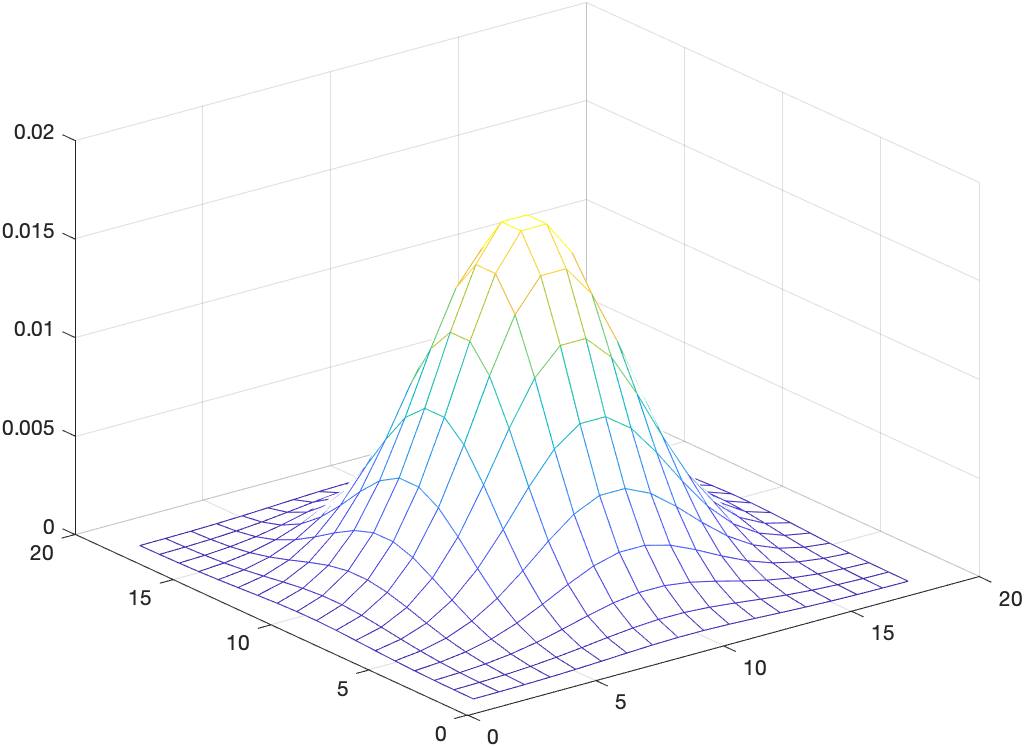
\includegraphics[width=1\columnwidth]{gaussian_kernel.png}
\caption[c1]{ 3D visualisation of a Gaussian kernel. }
\label{fig_1}
\end{figure}
 
 For image sharpening (high-pass filtering), we will present two types of kernels: the first derivative and second derivative kernels. First derivatives are usually used for detecting slopes in image values and second derivatives are used for detecting changes in slopes of values. For the first derivative, we usually use Roberts, Prewitt or Sobel kernels \ref{fig_10}, and for the second derivative, we use Laplacian kernels \ref{fig_11}.
 
 \begin{figure}[!htb]
\centering
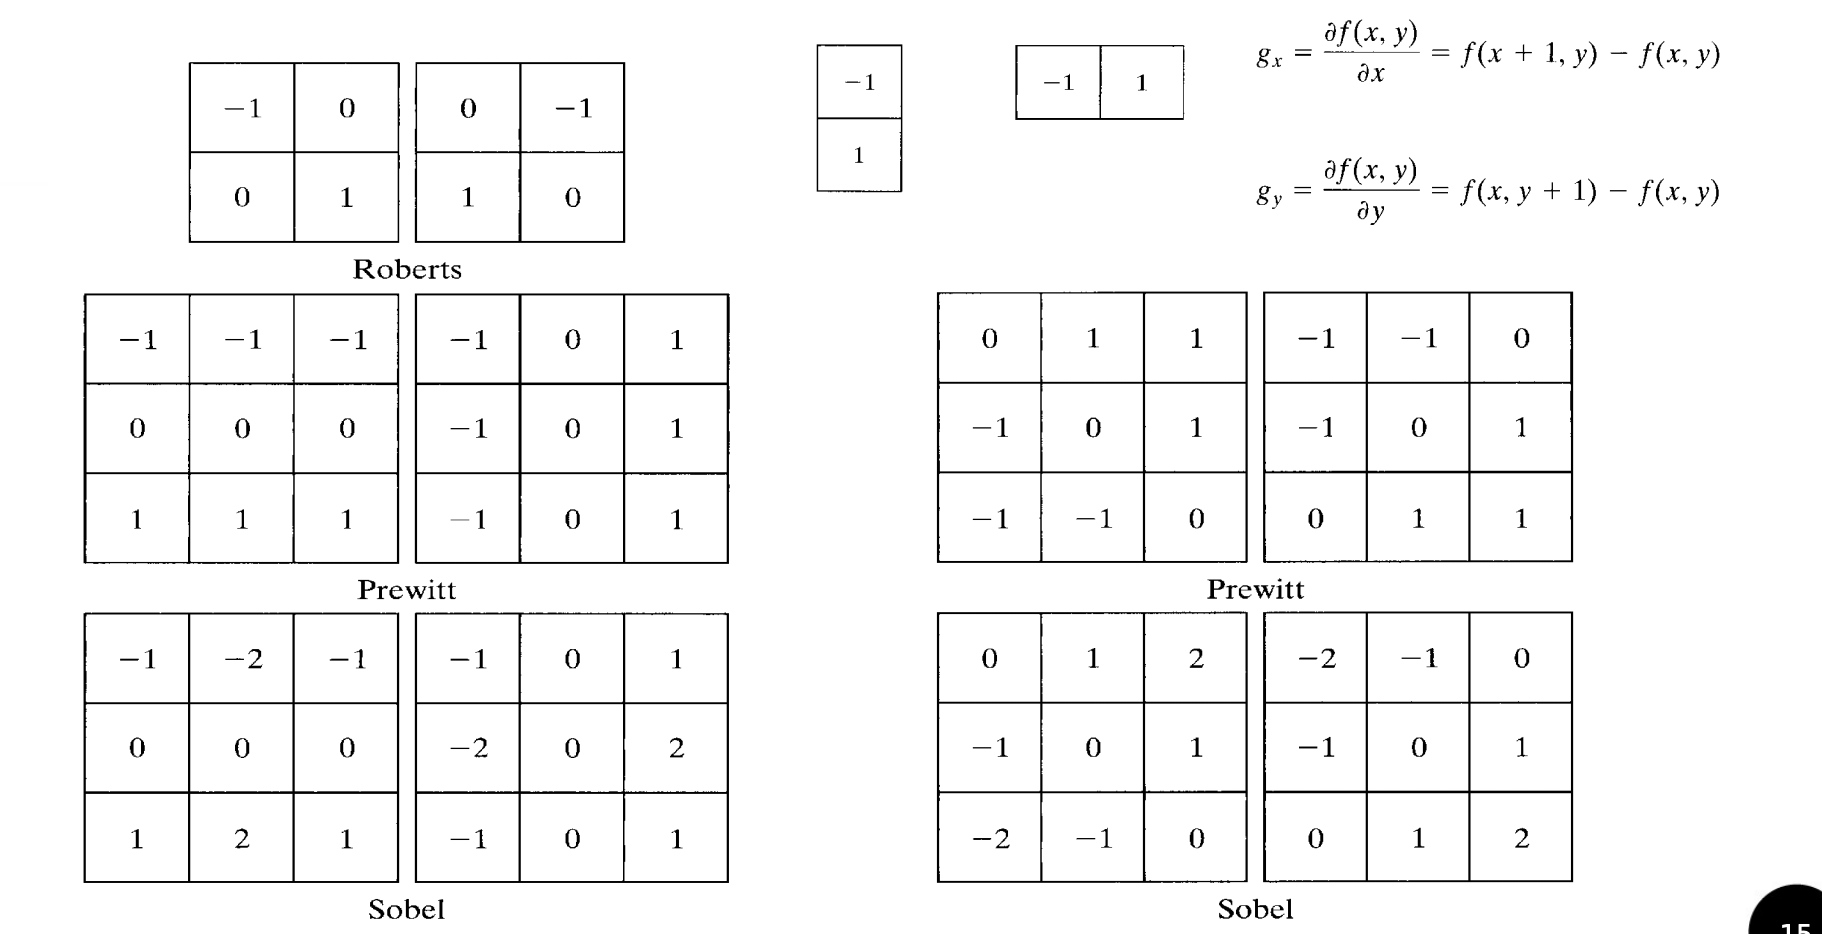
\includegraphics[width=1\columnwidth]{first_derivative_kernels.png}
\caption[c1]{ Examples of first derivative kernels. }
\label{fig_10}
\end{figure}
 
\begin{figure}[!htb]
\centering
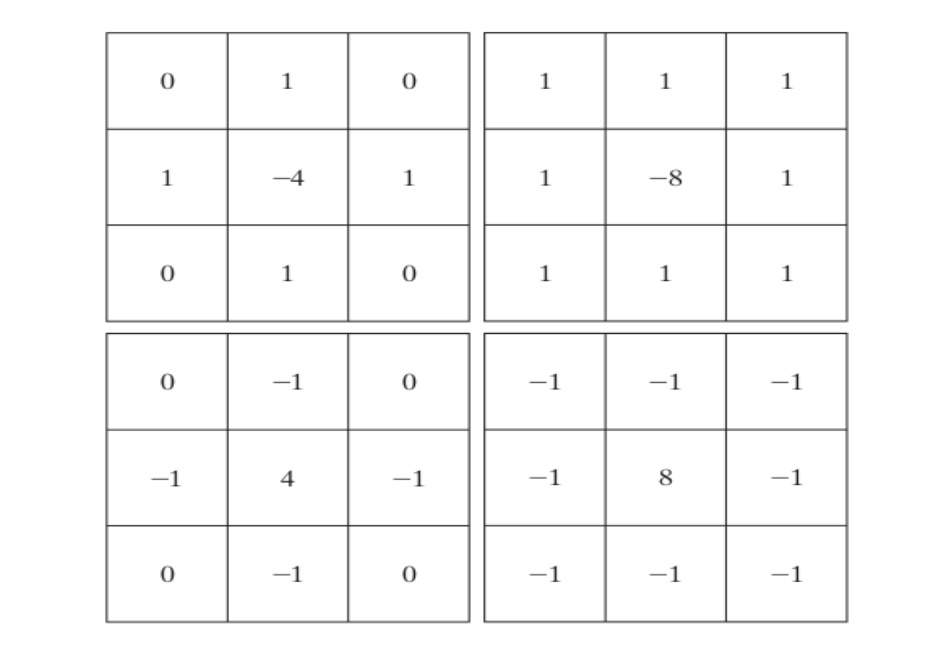
\includegraphics[width=1\columnwidth]{laplacian_kernels.png}
\caption[c1]{ Examples of Laplacian kernels. }
\label{fig_11}
\end{figure}

\section{Methodology}

In this assignment, we will be implementing the Canny edge detector in the MATLAB environment. To properly implement the Canny detector, we must implement the following steps:

\begin{enumerate}
\item Smooth the image with a Gaussian filter
\item Compute the gradient magnitude and angle images
\item Apply nonmaxima suppression to the gradient magnitude image
\item Use hysteresis thresholding and connectivity analysis to detect and link edges
\end{enumerate}


\subsection{Gaussian filter}
According to the list above, we first applied low-pass filtering to our input CT image using the Gaussian filter. We created a Gaussian kernel using the $fspecial()$ function in MATLAB, and we then filtered the image using the $imfilter()$ function. 

\subsection{Gradient magnitude and angle images}
Then, we needed to calculate the magnitude and angle images from our source image. To achieve that, we first needed to derive the image on the x and y coordinates. To get the x and y derivatives of the image ($g_x and g_y$), we used Prewitt kernels \ref{fig_2}. If we put both derivatives in a vector together, they represent the gradient of the image at any given point. We would then like to represent the gradients of the image as vectors in polar coordinates, with each gradient being represented as a combination of the vector amplitude and the vector angle \ref{fig_3}. We computed the magnitude and angle values for each pixel of our image according to the following formulas \ref{eq3, eq4}. While computing the magnitude is pretty straightforward in MATLAB, it is important to note that we used the function $atan2()$ to calculate the arctan values for our gradient angles. This function is used to ensure that the values of arctan range from $-\pi$ to $\pi$, to ensure that we get correct angles for all 4 quadrants out of the equation as output.

\begin{figure}[!htb]
\centering
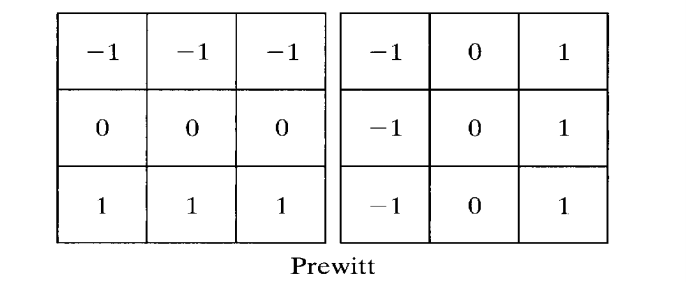
\includegraphics[width=1\columnwidth]{prewitt.png}
\caption[c1]{ Prewitt kernels to calculate the first derivative components of an image. }
\label{fig_2}
\end{figure}

\begin{figure}[!htb]
\centering
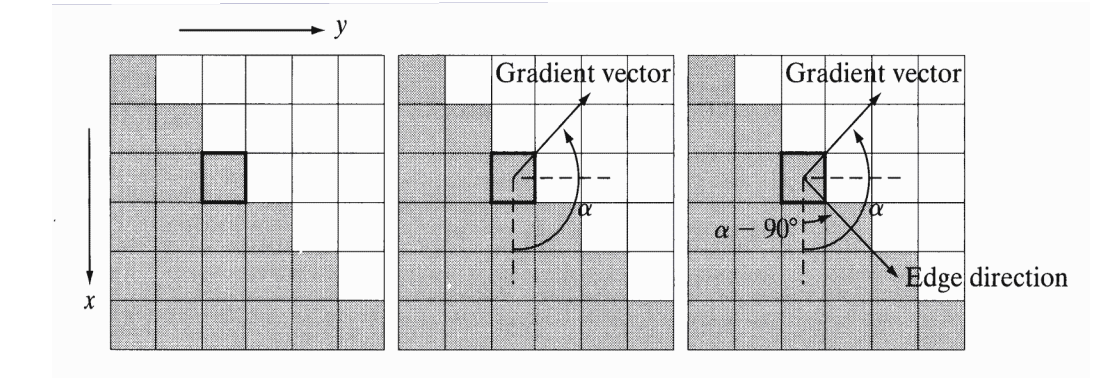
\includegraphics[width=1\columnwidth]{magnitude_angle.png}
\caption[c1]{ Edge gradient represented with a vector containing magnitude and angle attributes. }
\label{fig_3}
\end{figure}


\begin{equation} \label{eq3}
M[x, y] = mag(\nabla f) = \sqrt{g_x^2 + g_y^2}
 \end{equation}

 \begin{equation} \label{eq4}
\alpha[x, y] = tan^{-1}[\dfrac{g_y}{g_x}]
 \end{equation}

\subsection{Nonmaxima suppression}

The next step is nonmaxima suppression, a procedure applied to the magnitude image that removes unnecessary pixels in the gradient magnitudes image, based on the angle of the gradient. The procedure goes like this:

\begin{enumerate}
\item We define four basic directions (vertical, horizontal, -45 degree, 45 degree) that we get by dividing the circle into eight parts. For each pixel, we find the direction that most accurately describes the angle of the edge in the pixel. In our implementation, this is done by dividing the circle into eight equal parts, checking inside which of the parts is our angle, and assigning a direction based on the part of the circle that corresponds to the vector angle. It is important to note that the gradient angle represents the edge normal, the right angle of our edge, so we need to take that into account when deciding on the direction of our edge.
\item When we have the direction of our edge in each pixel, we calculate the new suppressed image values accordingly, by comparing magnitude values in the direction of the edge in a 3x3 grid around each pixel in the magnitude image. If the value of the magnitude pixel is less than any of the neighbouring values along the edge direction, we set the value of the suppressed image pixel at the same place as the centre magnitude pixel to 0. Otherwise, we set the new pixel value the same as the magnitude value at the same place.
\end{enumerate}

\begin{figure}[!htb]
\centering
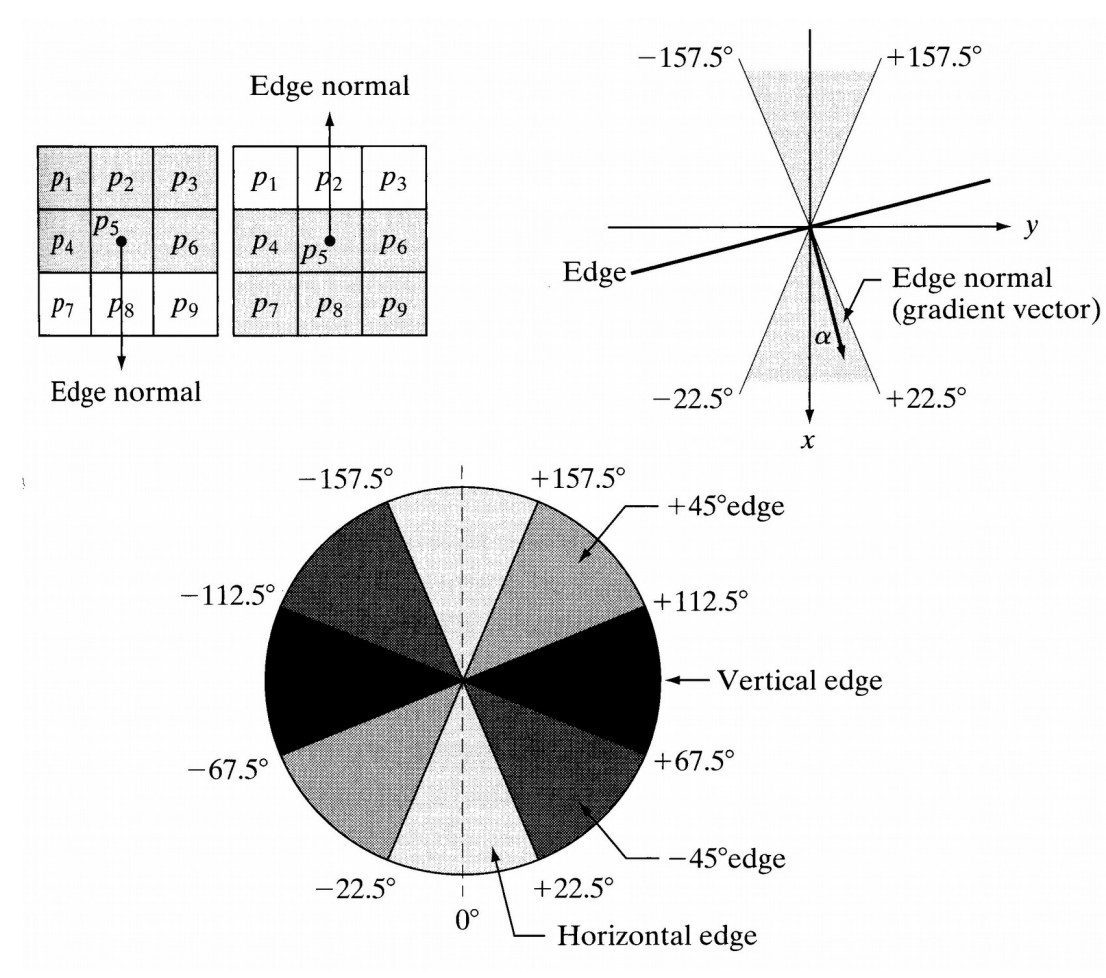
\includegraphics[width=1\columnwidth]{nonmaxima_suppression.png}
\caption[c1]{ Nonmaxima suppression procedure visualized. }
\label{fig_4}
\end{figure}

\subsection{Hysteresis thresholding}

The last step of the Canny edge detector is the hysteresis thresholding. It performs additional edge thinning, and also links together edges that might be disconnected. The steps for hysteresis thresholding are these:

\begin{enumerate}
\item We will use two thresholds: $TH$ and $TL$. We select $TH$ empirically, and then set $TL$ as $TL = \dfrac{TH}{2}$.
\item We then calculate two images: $g_{NH}$ for strong pixels, which contains pixels in our image that are above the high threshold $TH$, and $g_{NL}$ for weak pixels, pixels that are above the threshold $TL$ but below the threshold $TH$. We calculate $g_{NH}$  with the equation $g_{NH}(x,y) = image(x,y) >= TH$, and  $g_{NL}$ with the equation $g_{NL}(x, y) = (image(x, y) >= TL) - g_{NH}$.
\item We can then calculate the thresholded image. All of the non-zero values in the $g_{NH}$ can be instantly classified as valid pixels for our thresholded image.
\item For the non-zero values in the $g_{NL}$, their validity is calculated a bit differently. We need to iterate through all of the non-zero values in $g_{NH}$, and then search the 3x3 area around every non-zero value in $g_{NH}$. If there is a non-zero value for  $g_{NH}$ in the area around, we can classify this pixel as valid in our thresholded image. 
\end{enumerate}

After all these steps, we finally get the thresholded image, which represents our edges found in the input CT image with the Canny edge detector.

\section{Results}

To present the results of our implementation of the Canny edge detector, we will display the image after each step in the edge detection process for the image named $0090.png$ \ref{fig_5} in the CTMRI database.

\begin{figure}[!htb]
\centering
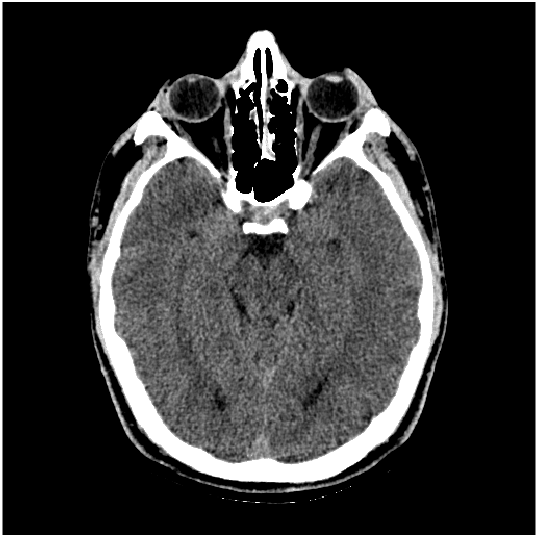
\includegraphics[width=0.8\columnwidth]{original_image.png}
\caption[c1]{ Our original input image. }
\label{fig_5}
\end{figure}

After the gaussian kernel filtering (with $\sigma = 2.5600$ and $kernelsize = 15$), we get the image  \ref{fig_6}.

\begin{figure}[!htb]
\centering
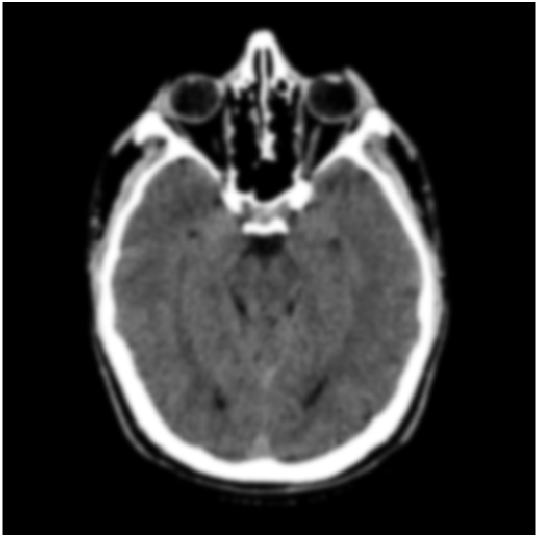
\includegraphics[width=0.8\columnwidth]{lp_filtered_image.png}
\caption[c1]{ Input image with the Gaussian filtering applied. }
\label{fig_6}
\end{figure}

Then we calculate the magnitude and angle images from our low-pass filtered image \ref{fig_7}.

\begin{figure}[!htb]
\centering
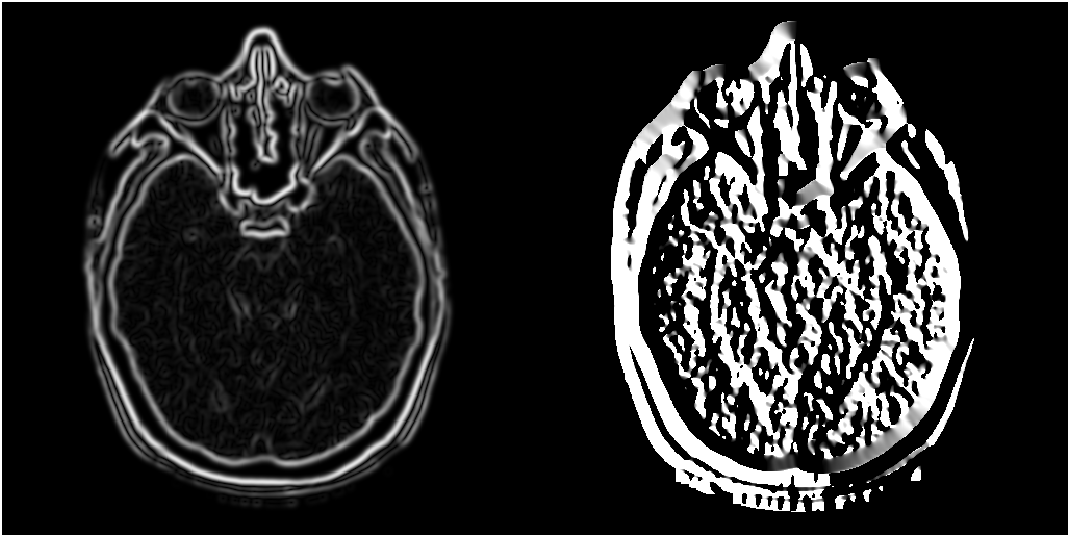
\includegraphics[width=0.8\columnwidth]{magnitudes_angles.png}
\caption[c1]{ Left part represents the magnitude image and the right part represents the angle image. }
\label{fig_7}
\end{figure}

We modify the magnitude image by performing nonmaxima supression \ref{fig_8}.

\begin{figure}[!t]
\centering
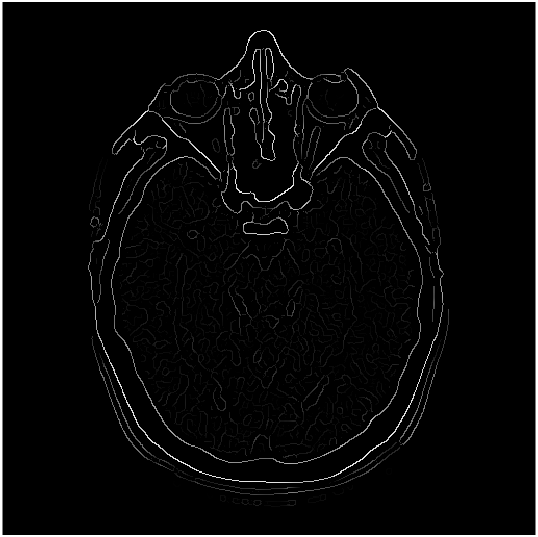
\includegraphics[width=0.8\columnwidth]{suppressed_image.png}
\caption[c1]{ The magnitudes image after nonmaxima supression. }
\label{fig_8}
\end{figure}


Finally, we perform hysteresis thresholding (with $TH = 0.1$ and $TL = 0.05$) on the nonmaxima supressed image, getting the final result of the Canny edge detector. \ref{fig_9}.

\begin{figure}[!t]
\centering
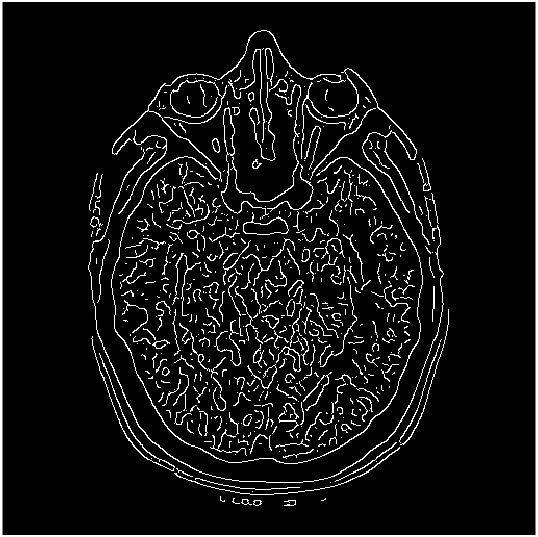
\includegraphics[width=0.8\columnwidth]{thresholded_image.png}
\caption[c1]{ The final image with edges detected. }
\label{fig_9}
\end{figure}

\section{Discussion}

While our Canny detector detects edges in CT images pretty well, there are many improvements that can be done to improve the performance. We could for example use better edge linking methods, or, instead of getting to $TH$ and $TL$ values empirically, using a more complex method for defining thresholds.

\FloatBarrier

\bibliographystyle{IEEEtran}
\bibliography{bibliography}

\end{document}